\newpage

\section{Attività di verifica}
In questa sezione del documento, vengono descritti e analizzati gli esiti delle attività di verifica svolte su tutti i documenti che vengono consegnati nelle varie revisioni di avanzamento del progetto.

\newpage
\section{Tracciamento}

\subsection{Tracciamento Test di Unità - Metodi}

% TABELLA
\normalsize
\begin{longtable}{|>{\centering}m{5cm}|m{5cm}<{\centering}|}
	\hline \rowcolor{Gray}
	\textbf{Test} & \textbf{Metodi}\\
	\hline
	\endhead
	
	\caption[Tracciamento Test di Unità-Metodi]{Tracciamento Test di Unità-Metodi}
	\label{tabella:tu-metodi}
\end{longtable}
\clearpage

\subsection{Tracciamento Metodi - Test di Unità}

% TABELLA
\normalsize
\begin{longtable}{|>{\centering}m{5cm}|m{5cm}<{\centering}|}
	\hline \rowcolor{Gray}
	\textbf{Metodi} & \textbf{Test}\\
	\hline
	\endhead
	
	\caption[Tracciamento Metodi-Test di Unità]{Tracciamento Metodi-Test di Unità}
	\label{tabella:metodi-tu}
\end{longtable}
\clearpage

\subsection{Tracciamento Test di Integrazione - Componenti}

% TABELLA
\normalsize
\begin{longtable}{|>{\centering}m{5cm}|m{7cm}<{\centering}|}
	\hline \rowcolor{Gray}
	\textbf{Test} & \textbf{Componenti}\\
	\hline
	\endhead
	\hyperlink{TI1}{TI1} & APIM::FrontEnd::Index \\ \hline
	\hyperlink{TI2}{TI2} & APIM::FrontEnd::App::Controllers \\ \hline
	\hyperlink{TI3}{TI3} & APIM::BackEnd::Services \\ \hline
	\hyperlink{TI4}{TI4} & APIM::FrontEnd::App::Models\\&APIM::BackEnd::Services \\ \hline
	\hyperlink{TI5}{TI5} & APIM::FrontEnd::App::Views\\&APIM::FrontEnd::Controllers \\ \hline
	\hyperlink{TI6}{TI6} & APIM::BackEnd::Services \\ \hline
	\hyperlink{TI7}{TI7} & APIM::FrontEnd::node\_modules\\&APIM::FrontEnd::App::AppRun \\ \hline
	\hyperlink{TI8}{TI8} & APIM::FrontEnd::App::AppRouter\\&APIM::BackEnd::Services\\&APIM::BackEnd::Gateway \\ \hline
	\hyperlink{TI9}{TI9} & APIM::FrontEnd::App::Controllers \\ \hline
	\hyperlink{TI10}{TI10} & APIM::FrontEnd::App::Models\\&APIM::FrontEnd::App::Controllers \\ \hline
	
	\caption[Tracciamento Test di Integrazione-Componenti]{Tracciamento Test di Integrazione-Componenti}
	\label{tabella:ti-componenti}
\end{longtable}
\clearpage

\subsection{Tracciamento Componenti - Test di Integrazione}

% TABELLA
\normalsize
\begin{longtable}{|>{\centering}m{5cm}|m{5cm}<{\centering}|}
	\hline \rowcolor{Gray}
	\textbf{Componenti} & \textbf{Test}\\
	\hline
	\endhead
	
	\caption[Tracciamento Componenti-Test di Integrazione]{Tracciamento Componenti-Test di Integrazione}
	\label{tabella:componenti-ti}
\end{longtable}
\clearpage

\subsection{Tracciamento Test di Sistema - Requisiti}

% TABELLA
\normalsize
\begin{longtable}{|>{\centering}m{5cm}|m{5cm}<{\centering}|}
	\hline \rowcolor{Gray}
	\textbf{Test} & \textbf{Requisito}\\
	\hline
	\endhead
	\hyperlink{TSFO1}{TSFO1} & RFO1\\ \hline
	\hyperlink{TSFO2}{TSFO2} & RFO2\\ \hline
	\hyperlink{TSFD3}{TSFD3} & RFD3\\ \hline
	\hyperlink{TSFO4}{TSFO4} & RFO4\\ \hline
	\hyperlink{TSFO4.3}{TSFO4.3} & RFO4.3\\ \hline
	\hyperlink{TSFO5}{TSFO5} & RFO5\\ \hline
	\hyperlink{TSFO5.6}{TSFO5.6} & RFO5.6\\ \hline
	\hyperlink{TSFO5.7}{TSFO5.7} & RFO5.7\\ \hline
	\hyperlink{TSFO6.2}{TSFO6.2} & RFO6.2\\ \hline
	\hyperlink{TSFO7}{TSFO7} & RFO7\\ \hline
	\hyperlink{TSFO7.5.3}{TSFO7.5.3} & RFO7.5.3\\ \hline
	\hyperlink{TSFO8}{TSFO8} & RFO8\\ \hline
	\hyperlink{TSFO8.2}{TSFO8.2} & RFO8.2\\ \hline
	\hyperlink{TSFO8.2.4}{TSFO8.2.4} & RFO8.2.4\\ \hline
	\hyperlink{TSFO8.2.8}{TSFO8.2.8} & RFO8.2.8\\ \hline
	\hyperlink{TSFO8.2.9}{TSFO8.2.9} & RFO8.2.9\\ \hline
	\hyperlink{TSFO9}{TSFO9} & RFO9\\ \hline
	\hyperlink{TSFO10.1}{TSFO10.1} & RFO10.1\\ \hline
	\hyperlink{TSFO10.1.1}{TSFO10.1.1} & RFO10.1.1\\ \hline
	\hyperlink{TSFO10.1.2}{TSFO10.1.2} & RFO10.1.2\\ \hline
	\hyperlink{TSFD10.1.2.9}{TSFD10.1.2.9} & RFD10.1.2.9\\ \hline
	\hyperlink{TSFO10.2}{TSFO10.2} & RFO10.2\\ \hline
	\hyperlink{TSFO10.2.1}{TSFO10.2.1} & RFO10.2.1\\ \hline
	\hyperlink{TSFO10.2.2}{TSFO10.2.2} & RFO10.2.2\\ \hline
	\hyperlink{TSFO10.3}{TSFO10.3} & RFO10.3\\ \hline
	\hyperlink{TSFO10.3.2}{TSFO10.3.2} & RFO10.3.2\\ \hline
	\hyperlink{TSFO11}{TSFO11} & RFO11\\ \hline
	\hyperlink{TSFO12.1.1.1}{TSFO12.1.1.1} & RFO12.1.1.1\\ \hline
	\hyperlink{TSFO12.1.1.2}{TSFO12.1.1.2} & RFO12.1.1.2\\ \hline
	\hyperlink{TSFD12.1.1.3}{TSFD12.1.1.3} & RFD12.1.1.3\\ \hline
	\hyperlink{TSFO12.2.1.1}{TSFO12.2.1.1} & RFO12.2.1.1\\ \hline
	\hyperlink{TSFO12.2.1.2}{TSFO12.2.1.2} & RFO12.2.1.2\\ \hline
	\hyperlink{TSFO12.2.1.3}{TSFO12.2.1.3} & RFO12.2.1.3\\ \hline
	\hyperlink{TSFO12.2.1.5}{TSFO12.2.1.5} & RFO12.2.1.5\\ \hline
	\hyperlink{TSVO1}{TSVO1} & RVO1\\ \hline
	\hyperlink{TSVO2}{TSVO2} & RVO2\\ \hline
	\hyperlink{TSVO3}{TSVO3} & RVO3\\ \hline
	\hyperlink{TSVO4}{TSVO4} & RVO4\\ \hline
	\hyperlink{TSVO5}{TSVO5} & RVO5\\ \hline
	\hyperlink{TSVO6}{TSVO6} & RVO6\\ \hline
	\hyperlink{TSVO7}{TSVO7} & RVO7\\ \hline
	\hyperlink{TSVD8}{TSVD8} & RVD8\\ \hline
	\hyperlink{TSVD9}{TSVD9} & RVD9\\ \hline
	\hyperlink{TSVO10}{TSVO10} & RVO10\\ \hline
	\hyperlink{TSVO11}{TSVO11} & RVO11\\ \hline
	\hyperlink{TSVO12}{TSVO12} & RVO12\\ \hline
	\hyperlink{TSVF13}{TSVF13} & RVF13\\ \hline
	\hyperlink{TSVD14}{TSVD14} & RVD14\\ \hline	
	\caption[Tracciamento Test di Sistema-Requisiti]{Tracciamento Test di Sistema-Requisiti}
	\label{tabella:ts-requi}
\end{longtable}
\clearpage

\subsection{Tracciamento Requisiti - Test di Sistema}

% TABELLA
\normalsize
\begin{longtable}{|>{\centering}m{5cm}|m{5cm}<{\centering}|}
	\hline \rowcolor{Gray}
	\textbf{Requisito} & \textbf{Test}\\
	\hline
	\endhead

	\caption[Tracciamento Requisiti-Test di Sistema]{Tracciamento Requisiti-Test di Sistema}
	\label{tabella:requi-ts}
\end{longtable}
\clearpage

\subsection{Tracciamento Test di Validazione - Requisiti}

% TABELLA
\normalsize
\begin{longtable}{|>{\centering}m{5cm}|m{5cm}<{\centering}|}
	\hline \rowcolor{Gray}
	\textbf{Test} & \textbf{Requisito}\\
	\hline
	\endhead
	\hyperlink{TVFO1}{TVFO1} & RFO1\\ \hline
	\hyperlink{TVFO2}{TVFO2} & RFO2\\ \hline
	\hyperlink{TVFO4}{TVFO4} & RFO4\\ \hline
	\hyperlink{TVFO5}{TVFO5} & RFO5\\ \hline
	\hyperlink{TVFO5.6}{TVFO5.6} & RFO5.6\\ \hline
	\hyperlink{TVFO7}{TVFO7} & RFO7\\ \hline
	\hyperlink{TVFO8.2}{TVFO8.2} & RFO8.2\\ \hline
	\hyperlink{TVFO8.2.3}{TVFO8.2.3} & RFO8.2.3\\ \hline
	\hyperlink{TVFO8.2.4}{TVFO8.2.4} & RFO8.2.4\\ \hline
	\hyperlink{TVFO9}{TVFO9} & RFO9\\ \hline
	\hyperlink{TVFO10.1.1}{TVFO10.1.1} & RFO10.1.1\\ \hline
	\hyperlink{TVFO10.1.2}{TVFO10.1.2} & RFO10.1.2\\ \hline
	\hyperlink{TVFD10.1.2.9}{TVFD10.1.2.9} & RFO10.1.2.9\\ \hline
	\hyperlink{TVFO10.2.1}{TVFO10.2.1} & RFO10.2.1\\ \hline
	\hyperlink{TVFO10.3}{TVFO10.3} & RFO10.3\\ \hline
	\hyperlink{TVFO11}{TVFO11} & RFO11\\ \hline
	\hyperlink{TVFO12.2.1}{TVFO12.2.1} & RFO12.2.1\\ \hline
	\caption[Tracciamento Test di Validazione-Requisiti]{Tracciamento Test di Validazione-Requisiti}
	\label{tabella:tv-requi}
\end{longtable}
\clearpage


\subsection{Resoconto verifica documenti}

L’analisi dei documenti mediante la tecnica \textit{Walkthrough} ha reso possibile individuare alcuni errori frequenti, che si sono aggiunti alla lista di controllo stilata ed aggiornata nelle varie revisioni, utile per applicare la tecnica \textit{Inspection} nelle future attività di verifica.\\
Il team, attraverso il software interno \textit{NetBreakDB}, è riuscito ad effettuare i tracciamenti per le componenti di interesse previste da ogni revisione (casi d’uso-requisiti, requisiti-fonti, requisiti-componenti, requisiti-classi, etc.).\\
Inoltre, questo software è stato utilizzato per generare le tabelle dei vari test e dei relativi tracciamenti con requisiti, componenti, classi e metodi.
	
	\subsection{Revisione dei Requisiti}
	Di seguito, sono riportati gli esiti delle verifiche sottoposte a tutti i documenti, per il calcolo della metrica \textit{Indice Gulpease} (\hyperlink{MPC19}{MPC19}).
	
		\begin{longtable}{|>{\centering\arraybackslash}p{5.5cm}|>{\centering\arraybackslash}p{5cm} | >{\centering\arraybackslash}p{5cm}|}
			\hline
			\rowcolor{Gray}
			\textbf{Documento} & \textbf{Indice Gulpease} & \textbf{Esito} \\
			\hline
			\textit{\NdP\ 1.0.0} & 49 & \textcolor{Green}{\textit{Superato}}\\
			\hline
			\textit{\PdP\ 1.0.0} & 50 & \textcolor{Green}{\textit{Superato}} \\
			\hline
			\textit{\PdQ\ 1.0.0} & 42 & \textcolor{Green}{\textit{Superato}}\\
			\hline
			\textit{\AdR\ 1.0.0} & 68 & \textcolor{Green}{\textit{Superato}} \\
			\hline
			\textit{\SdF\ 1.0.0} & 54 & \textcolor{Green}{\textit{Superato}}\\
			\hline
			\textit{\G\ 1.0.0}& 43 & \textcolor{Green}{\textit{Superato}}\\
			\hline
			\textit{Verbale Interno - 28/11/2016}		& 	60	&	\textcolor{Green}{\textit{Superato}}	\\
			\hline
			\textit{Verbale Interno - 01/12/2016}		& 	63	&	\textcolor{Green}{\textit{Superato}}	\\
			\hline
			\textit{Verbale Interno - 12/12/2016}		& 	61	&	\textcolor{Green}{\textit{Superato}}	\\
			\hline
			\textit{Verbale Esterno - 22/12/2016}		& 	59	&	\textcolor{Green}{\textit{Superato}}	\\
			\hline
			\textit{Verbale Interno - 28/12/2016}		& 	61	&	\textcolor{Green}{\textit{Superato}}	\\
			\hline
		
		\caption{Resoconto verifiche documenti - RR}
	\end{longtable}

\newpage	
	\subsection{Revisione di Progettazione}
	Di seguito, sono riportati gli esiti delle verifiche sottoposte a tutti i documenti, per il calcolo della metrica \textit{Indice Gulpease} (\hyperlink{MPC19}{MPC19}).
	
			\begin{longtable}{|>{\centering\arraybackslash}p{5.5cm}|>{\centering\arraybackslash}p{5cm} | >{\centering\arraybackslash}p{5cm}|}
				\hline
				\rowcolor{Gray}
				\textbf{Documento} & \textbf{Indice Gulpease} & \textbf{Esito} \\
				\hline
				\textit{\ST\ 1.0.0} & 67  & \textcolor{Green}{\textit{Superato}}\\
				\hline
				\textit{\NdP\ 2.0.0} & 57  & \textcolor{Green}{\textit{Superato}}\\
				\hline
				\textit{\PdP\ 2.0.0} & 55 & \textcolor{Green}{\textit{Superato}} \\
				\hline
				\textit{\PdQ\ 2.0.0} & 54  & \textcolor{Green}{\textit{Superato}}\\
				\hline
				\textit{\AdR\ 2.0.0} & 70  & \textcolor{Green}{\textit{Superato}} \\
				\hline
				\textit{\G\ 2.0.0}& 49 & \textcolor{Green}{\textit{Superato}}\\
				\hline
				\textit{Verbale Interno - 27/01/2017}		& 	55	&	\textcolor{Green}{\textit{Superato}}	\\
				\hline
				\textit{Verbale Interno - 04/02/2017}		& 	64	&	\textcolor{Green}{\textit{Superato}}	\\
				\hline
				\textit{Verbale Interno - 13/02/2017}		& 	58	&	\textcolor{Green}{\textit{Superato}}	\\
				\hline
				\textit{Verbale Esterno - 16/02/2017}		& 	60	&	\textcolor{Green}{\textit{Superato}}	\\
				\hline
				\textit{Verbale Interno - 17/02/2017}		& 	57	&	\textcolor{Green}{\textit{Superato}}	\\
				\hline
				\textit{Verbale Interno - 21/02/2017}		& 	63	&	\textcolor{Green}{\textit{Superato}}	\\
				\hline
				\textit{Verbale Interno - 02/03/2017}		& 	61	&	\textcolor{Green}{\textit{Superato}}	\\
				\hline
				\textit{Verbale Interno - 03/03/2017}		& 	61	&	\textcolor{Green}{\textit{Superato}}	\\
				\hline
			
			\caption{Resoconto verifiche documenti - RP}
		\end{longtable}

\newpage
	\subsection{Revisione di Qualifica}
	Di seguito, sono riportati gli esiti delle verifiche sottoposte a tutti i documenti, per il calcolo della metrica \textit{Indice Gulpease} (\hyperlink{MPC19}{MPC19}).
	
			\begin{longtable}{|>{\centering\arraybackslash}p{5.7cm}|>{\centering\arraybackslash}p{5cm} | >{\centering\arraybackslash}p{5cm}|}
				\hline
				\rowcolor{Gray}
				\textbf{Documento} & \textbf{Indice Gulpease} & \textbf{Esito} \\
				\hline
				\textit{\DDP\ 1.0.0} & 72 & \textcolor{Green}{\textit{Superato}}\\
				\hline
				\textit{\MU\ 1.0.0} & 68 & \textcolor{Green}{\textit{Superato}}\\
				\hline
				\textit{\ST\ 2.0.0} & 69  & \textcolor{Green}{\textit{Superato}}\\
				\hline
				\textit{\NdP\ 3.0.0} & 61  & \textcolor{Green}{\textit{Superato}}\\
				\hline
				\textit{\PdP\ 3.0.0} & 60 & \textcolor{Green}{\textit{Superato}} \\
				\hline
				\textit{\PdQ\ 3.0.0} &  63 & \textcolor{Green}{\textit{Superato}}\\
				\hline
				\textit{\AdR\ 3.0.0} &  71 & \textcolor{Green}{\textit{Superato}} \\
				\hline
				\textit{\G\ 3.0.0}& 50 & \textcolor{Green}{\textit{Superato}}\\
				\hline
				\textit{Tracciamento Verbali Interni RQ}		& 	68	&	\textcolor{Green}{\textit{Superato}}	\\
				\hline
				\textit{Tracciamento Verbali Esterni RQ}		& 	67	&	\textcolor{Green}{\textit{Superato}}	\\
				\hline
				\textit{Verbale Interno 2017-03-16}		& 	57	&	\textcolor{Green}{\textit{Superato}}	\\
				\hline
				\textit{Verbale Interno 2017-03-31}		& 	61	&	\textcolor{Green}{\textit{Superato}}	\\
				\hline
				\textit{Verbale Interno 2017-04-28}		& 	59	&	\textcolor{Green}{\textit{Superato}}	\\
				\hline
				\textit{Verbale Esterno 2017-03-17}		& 	60	&	\textcolor{Green}{\textit{Superato}}	\\
				\hline
				\textit{Verbale Esterno 2017-03-30}		& 	65	&	\textcolor{Green}{\textit{Superato}}	\\
				\hline
				\textit{Verbale Esterno 2017-04-06}		& 	62	&	\textcolor{Green}{\textit{Superato}}	\\
				\hline
				\textit{Verbale Esterno 2017-04-10}		& 	64	&	\textcolor{Green}{\textit{Superato}}	\\
				\hline
				\textit{Verbale Esterno 2017-04-13}		& 	61	&	\textcolor{Green}{\textit{Superato}}	\\
				\hline
				\textit{Verbale Esterno 2017-04-19}		& 	65	&	\textcolor{Green}{\textit{Superato}}	\\
				\hline
				\textit{Verbale Esterno 2017-04-24}		& 	59	&	\textcolor{Green}{\textit{Superato}}	\\
				\hline

			\caption{Resoconto verifiche documenti - RQ}
		\end{longtable}

\newpage
\subsection{Revisione di Accettazione}
Di seguito, sono riportati gli esiti delle verifiche sottoposte a tutti i documenti, per il calcolo della metrica \textit{Indice Gulpease} (\hyperlink{MPC19}{MPC19}).

\begin{longtable}{|>{\centering\arraybackslash}p{5.7cm}|>{\centering\arraybackslash}p{5cm} | >{\centering\arraybackslash}p{5cm}|}
	\hline
	\rowcolor{Gray}
	\textbf{Documento} & \textbf{Indice Gulpease} & \textbf{Esito} \\
	\hline
	\textit{\DDP\ 2.0.0} & 73 & \textcolor{Green}{\textit{Superato}}\\
	\hline
	\textit{\MU\ 2.0.0} & 72 & \textcolor{Green}{\textit{Superato}}\\
	\hline
	\textit{\MS\ 1.0.0} & xx & \textcolor{Green}{\textit{Superato}}\\
	\hline
	\textit{\ST\ 3.0.0} & 70  & \textcolor{Green}{\textit{Superato}}\\
	\hline
	\textit{\NdP\ 4.0.0} & 65  & \textcolor{Green}{\textit{Superato}}\\
	\hline
	\textit{\PdP\ 4.0.0} & 63 & \textcolor{Green}{\textit{Superato}} \\
	\hline
	\textit{\PdQ\ 4.0.0} & 66 & \textcolor{Green}{\textit{Superato}}\\
	\hline
	\textit{\AdR\ 3.0.0} & 71 & \textcolor{Green}{\textit{Superato}} \\
	\hline
	\textit{\G\ 3.0.0}& 50 & \textcolor{Green}{\textit{Superato}}\\
	\hline
	\textit{Verbale Interno 2017-xx-yy}		& 	xx	&	\textcolor{Green}{\textit{Superato}}	\\
	\hline
	\textit{Verbale Esterno 2017-xx-yy}		& 	xx	&	\textcolor{Green}{\textit{Superato}}	\\
	\hline
	\textit{Verbale Interno 2017-xx-yy}		& 	xx	&	\textcolor{Green}{\textit{Superato}}	\\
	\hline
	
	\caption{Resoconto verifiche documenti - RA}
\end{longtable}

\subsection{Riepilogo}
Infine, per ogni documento principale, viene riportato un grafico che mostra la progressione e il rispettivo miglioramento del documento secondo l'\textit{indice Gulpease}.

\begin{figure}[H]
	\centering
	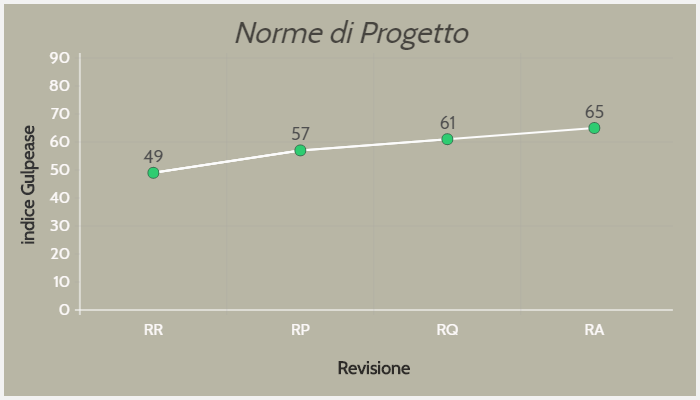
\includegraphics[scale=0.6]{includes/img/NdP.png}
	\caption{Miglioramento Norme di Progetto}
\end{figure}

\begin{figure}[H]
	\centering
	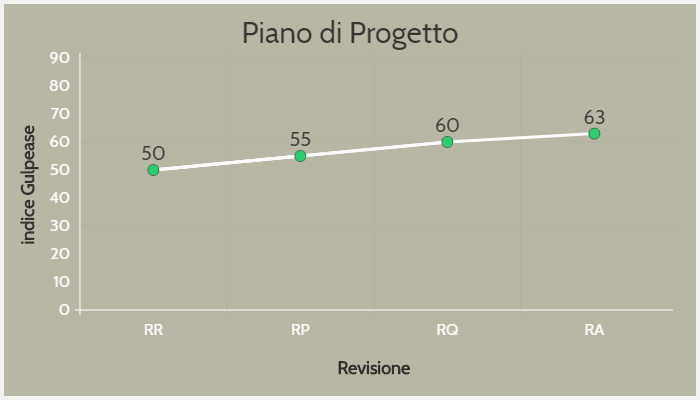
\includegraphics[scale=0.6]{includes/img/PdP.png}
	\caption{Miglioramento Piano di Progetto}
\end{figure}

\begin{figure}[H]
	\centering
	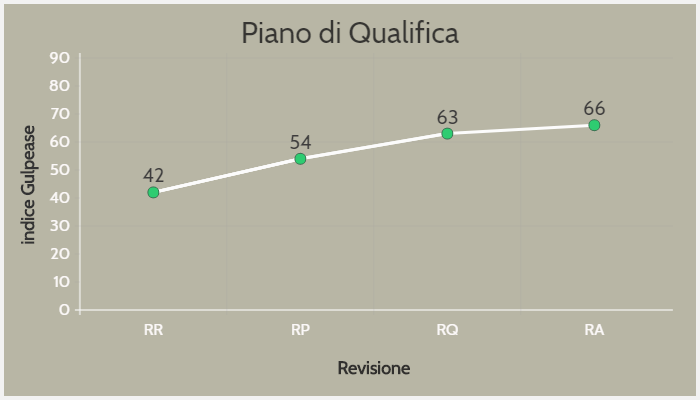
\includegraphics[scale=0.6]{includes/img/PdQ.png}
	\caption{Miglioramento Piano di Qualifica}
\end{figure}

\begin{figure}[H]
	\centering
	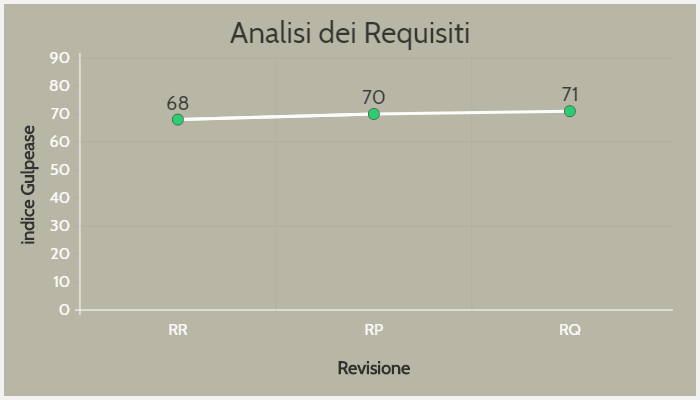
\includegraphics[scale=0.6]{includes/img/AdR.png}
	\caption{Miglioramento Analisi dei Requisiti}
\end{figure}

\begin{figure}[H]
	\centering
	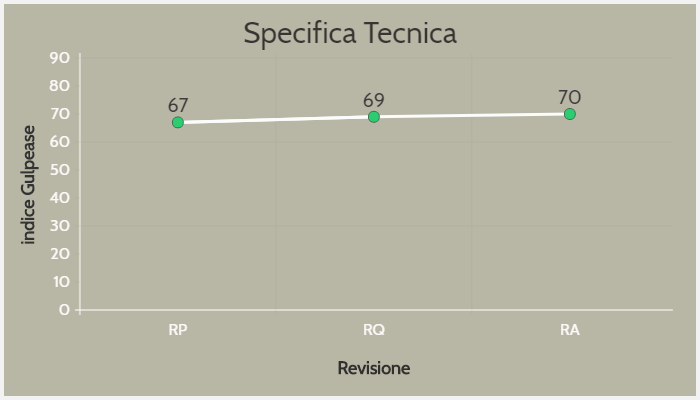
\includegraphics[scale=0.6]{includes/img/ST.png}
	\caption{Miglioramento Specifica Tecnica}
\end{figure}

\begin{figure}[H]
	\centering
	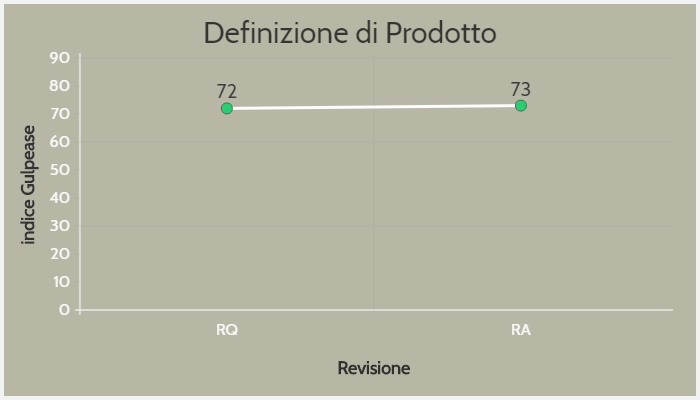
\includegraphics[scale=0.6]{includes/img/DDP.png}
	\caption{Miglioramento Definizione di Prodotto}
\end{figure}

\begin{figure}[H]
	\centering
	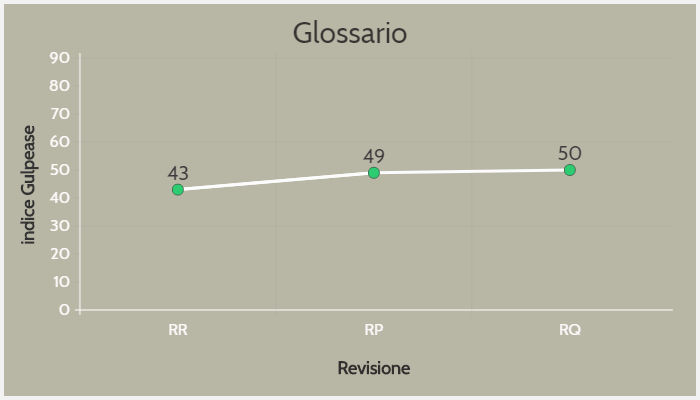
\includegraphics[scale=0.6]{includes/img/G.png}
	\caption{Miglioramento Glossario}
\end{figure}